\documentclass{article}
\usepackage{graphicx} % Required for inserting images
\usepackage{pdfpages}

\title{VM252$^*$ Logisim computer}
\author{Supreme Paudel}
\date{CS375}
\begin{document}

\maketitle

\tableofcontents
\section{Introduction}
VM252$^*$ Logisim circuit is a multi clock cycle CPU design that simulates the VM252 assembly language instructions. \newline
The multi-clock cycle VM252$^*$ model can be seen below:\newline
\newline
{\small Look at \textit{VM252ArchitectureSoftwareAndProgrammingInformation.pdf}
file inside the \textit{resources} directory in the github repository to learn about the VM252 Assembly language in detail. }

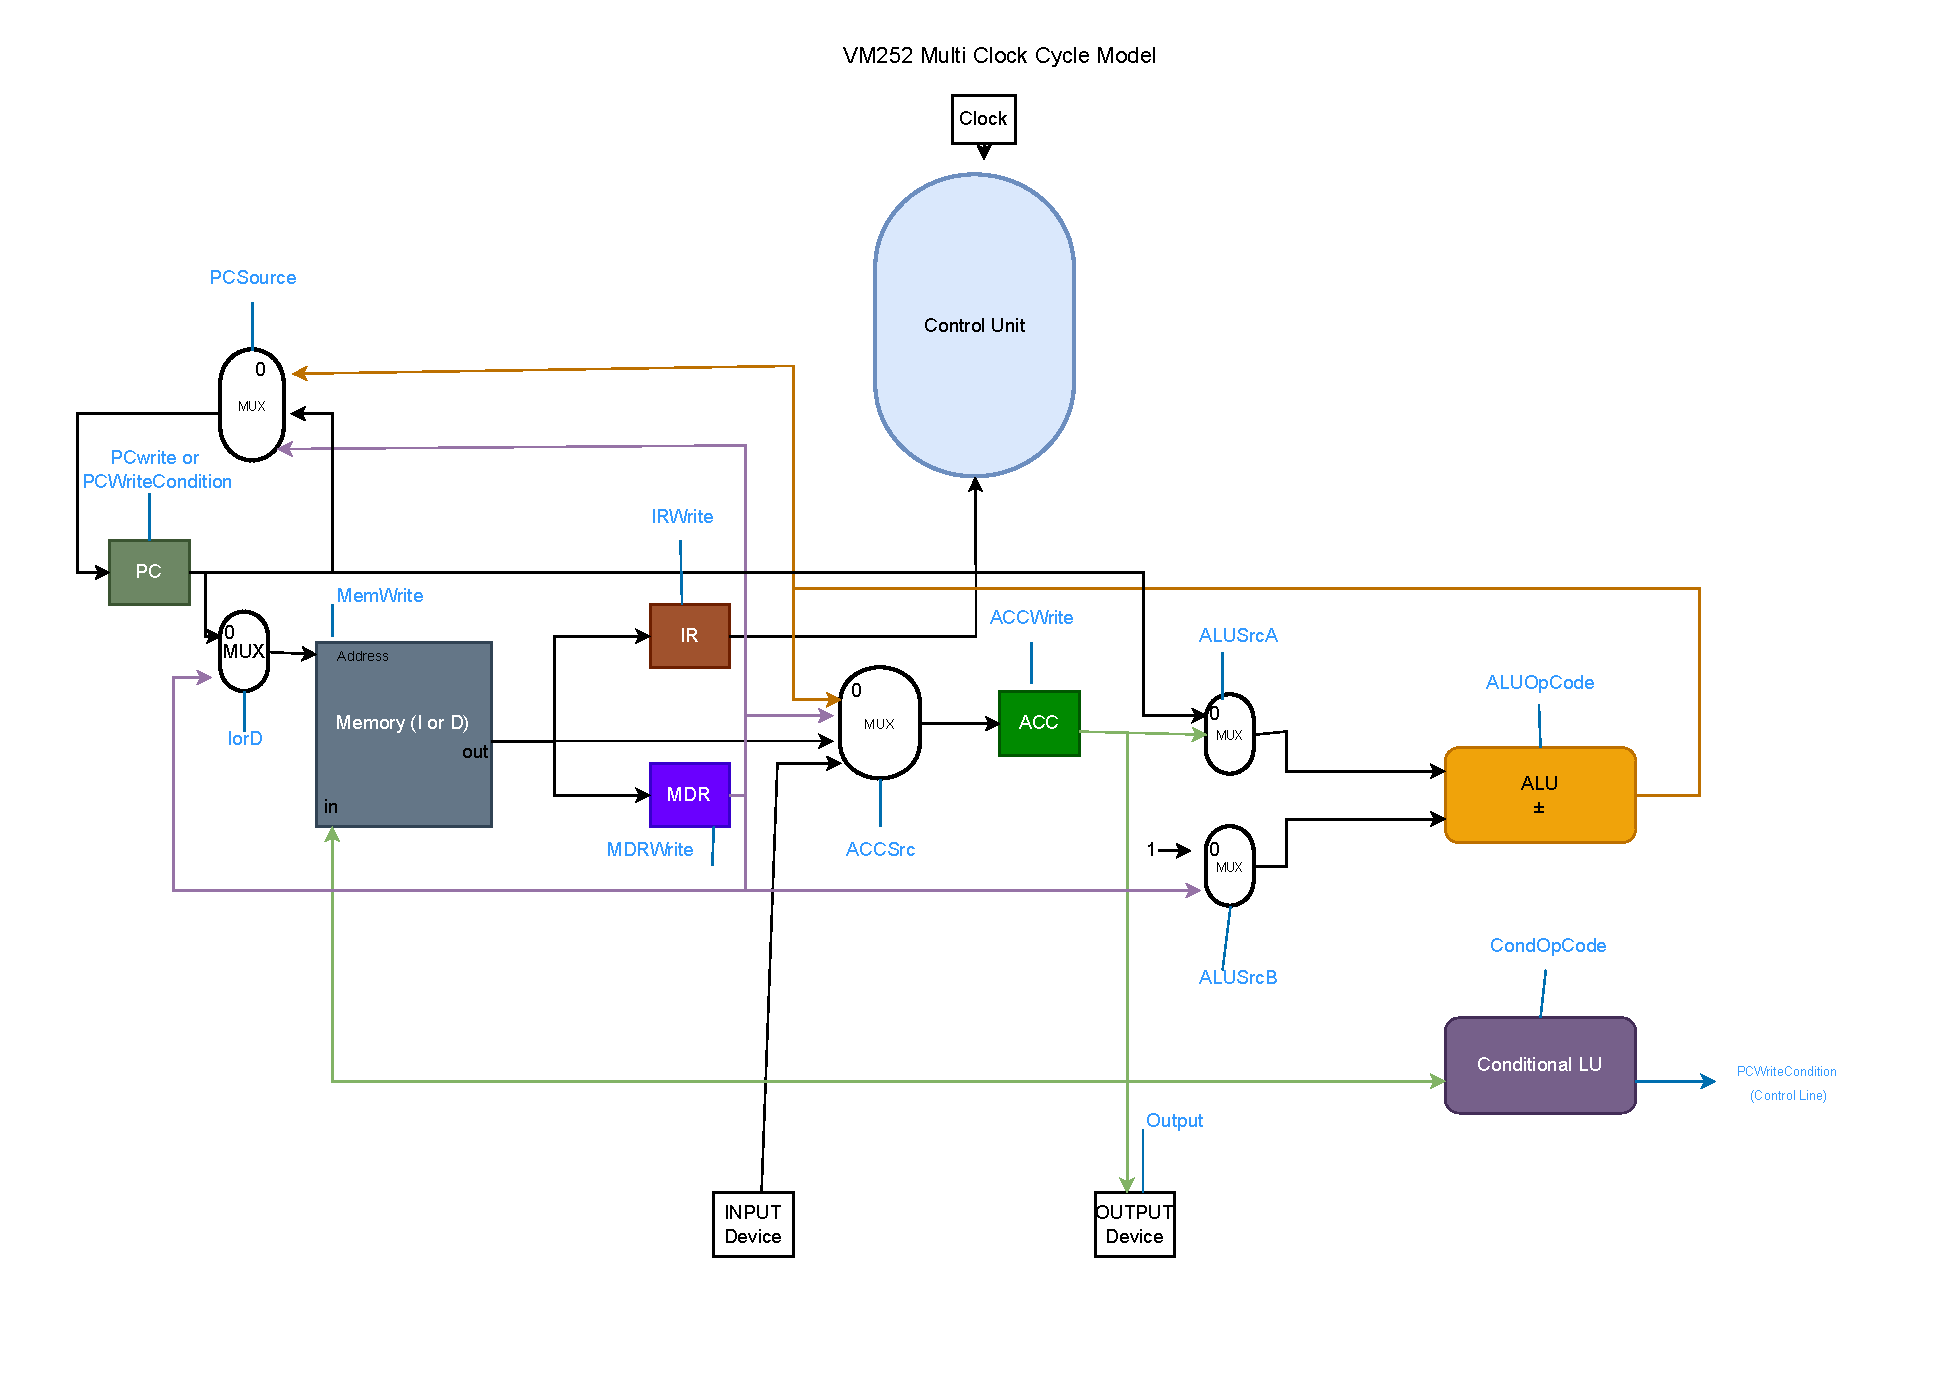
\includepdf[]{VM252Model.pdf}
The blue lines are the control lines coming from the control unit and have been omitted in this diagram. Moreover, some bit extenders and setting certain bits to 0 for memory addresses have not be shown in the diagram either.

\section{Why VM252$^*$ and not VM252?}

    \begin{enumerate}
        \item The VM252 memory is collection of 8192 eight-bit bytes whereas the VM252$^*$ memory is 8192 cells of size 16 bits each.
        \item All instructions in the VM252$^*$ are 16 bits long unlike the VM252 language where certain instructions are only 8 bits long.
        \item The Program Counter is always incremented by 1 to execute the next instruction unlike the VM252 because of (2).
    \end{enumerate}


\section{Instructions encoding}
\begin{itemize}
    \item Instructions are encoded in the same way as it is in the VM252 language except for the one big difference that $INPUT$, $OUTPUT$, $NOOP$ and $STOP$ instructions are now extended to be 16 bits instructions.
    \item The table below shows how the instructions are encoded and their respective hexadecimal value with the unknown bits set to 0: 
    \begin{center}
\begin{tabular}{ |c|c|c| } 
 \hline
 {\small Instruction} & {\small Instruction encoded in 16 bits} & {\small Hex value with unknown bits set to 0} \\ 
\hline
INPUT                                              & 111100xxxxxxxxxx                                       & F000                                                                  \\
OUTPUT                                             & 111101xxxxxxxxxx                                       & F400                                                                  \\
NOOP                                               & 111110xxxxxxxxxx                                       & F800                                                                  \\
STOP                                               & 111111xxxxxxxxxx                                       & FC00                                                                  \\
LOAD a                                             & 000$a_{12}a_{11}a_{10}a_9a_8a_7a_6a_5a_4a_3a_2a_1a_0$                                       & 0000                                                                  \\
STORE a                                            & 001$a_{12}a_{11}a_{10}a_9a_8a_7a_6a_5a_4a_3a_2a_1a_0$                                       & 2000                                                                  \\
ADD a                                              & 010$a_{12}a_{11}a_{10}a_9a_8a_7a_6a_5a_4a_3a_2a_1a_0$                                       & 4000                                                                  \\
SUB a                                              & 011$a_{12}a_{11}a_{10}a_9a_8a_7a_6a_5a_4a_3a_2a_1a_0$                                       & 6000                                                                  \\
JUMP a                                             & 100$a_{12}a_{11}a_{10}a_9a_8a_7a_6a_5a_4a_3a_2a_1a_0$                                       & 8000                                                                  \\
JUMPZ a                                            & 101$a_{12}a_{11}a_{10}a_9a_8a_7a_6a_5a_4a_3a_2a_1a_0$                                       & A000                                                                  \\
JUMPP a                                            & 110$a_{12}a_{11}a_{10}a_9a_8a_7a_6a_5a_4a_3a_2a_1a_0$                                       & C000                                                                  \\
SET c                                              & 1110$c_{11}c_{10}c_9c_8c_7c_6c_5c_4c_3c_2c_1c_0$                                       & E000        \\
 \hline
\end{tabular}
\end{center}
\item For example, a STORE instruction in address $9_{hex}$ would have hex value 2009.
\end{itemize}


\section{Finite State machine for the VM252$^*$}
For our multi-clock cycle design, we will need to implement a FSM to specify control. The FSM for our VM252$^*$ is shown below :
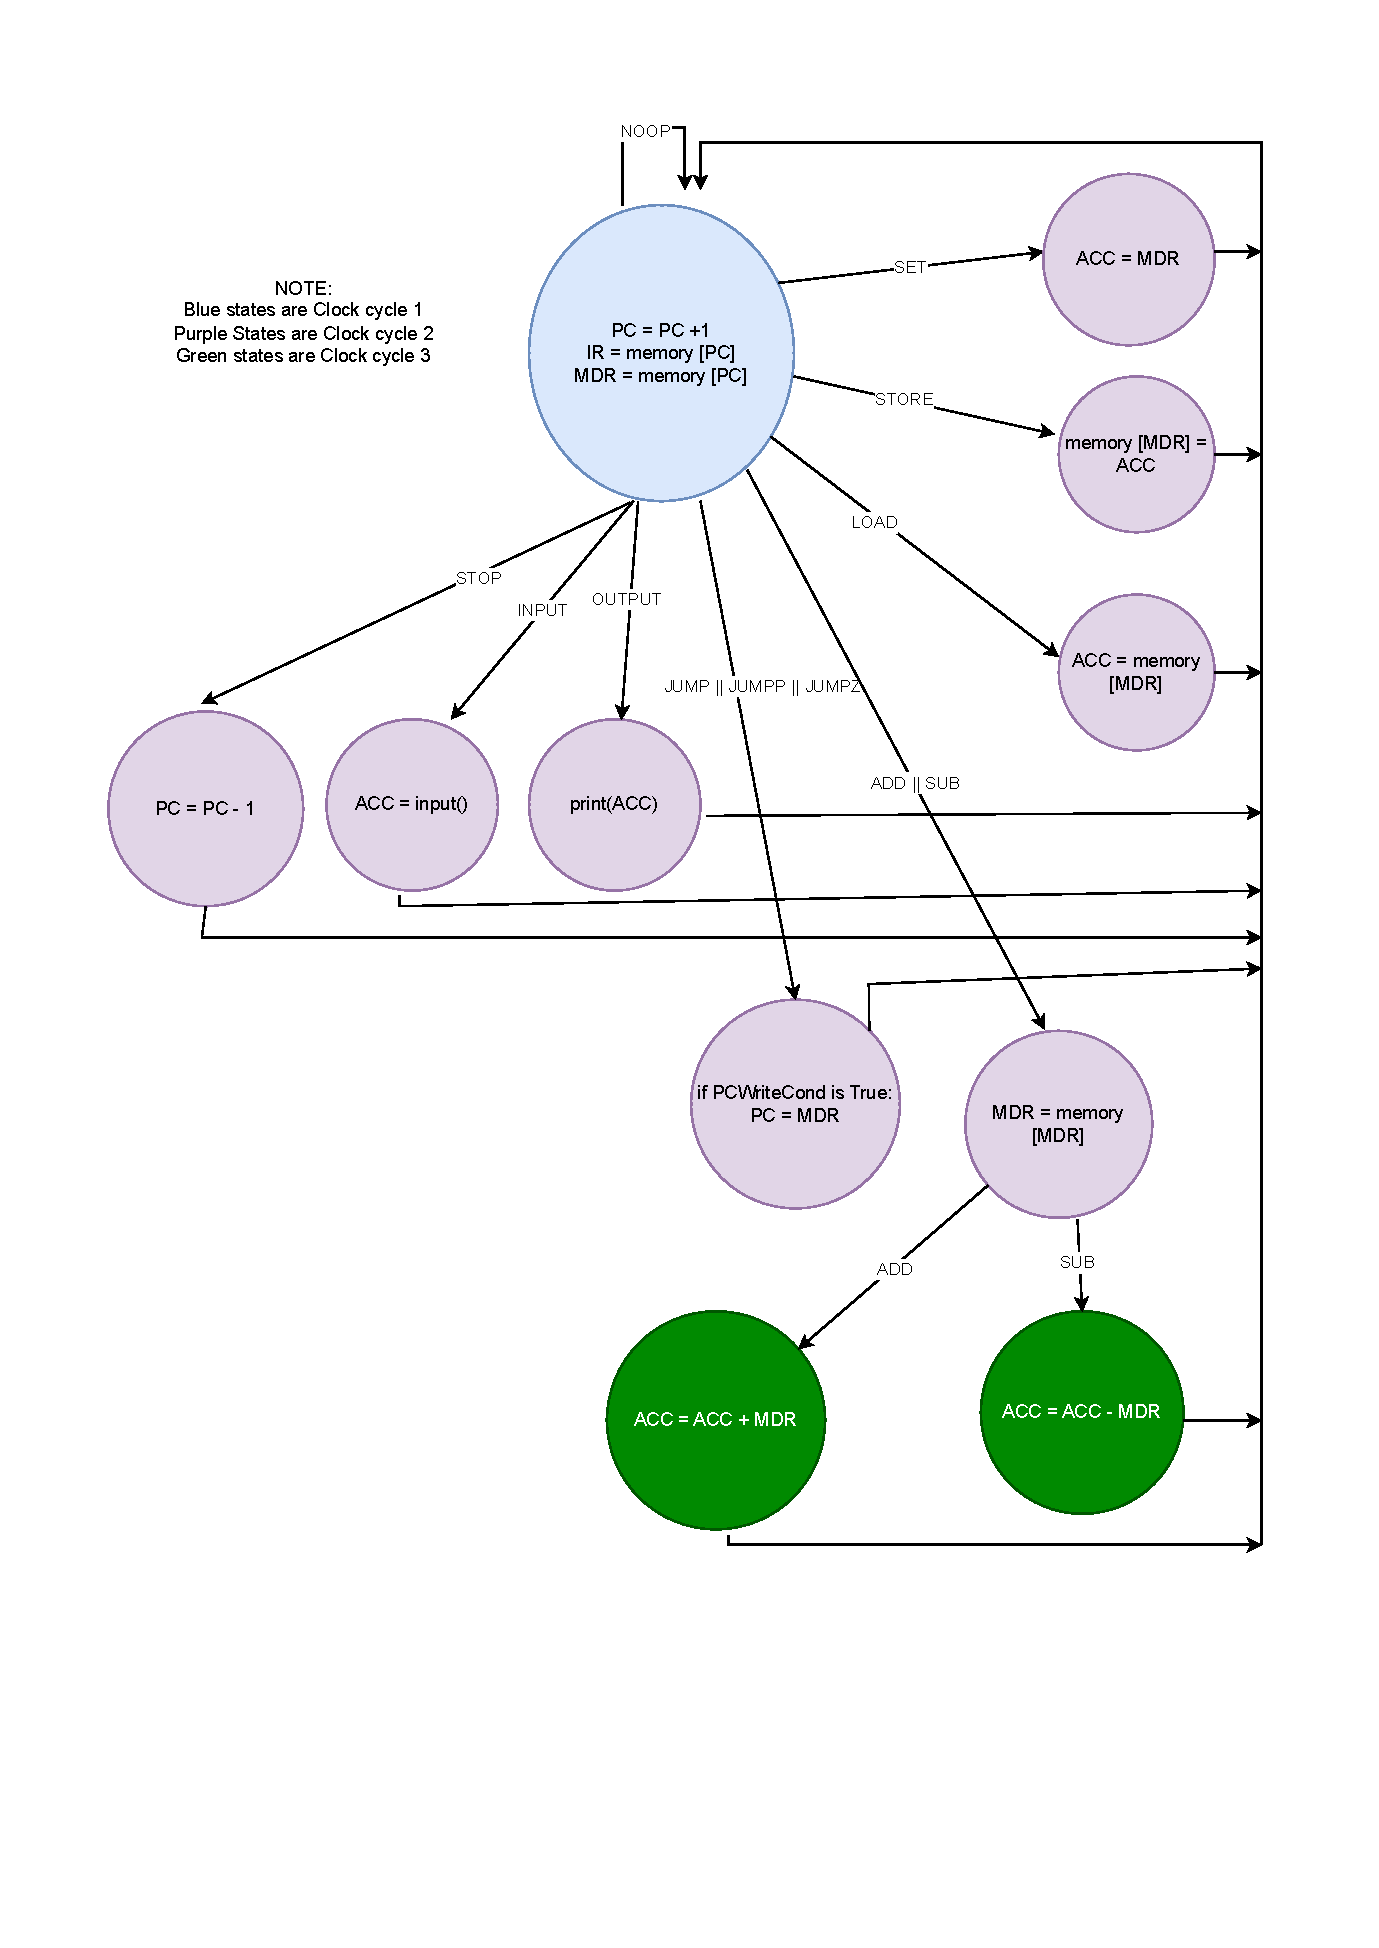
\includepdf[]{VM252FSM.pdf}
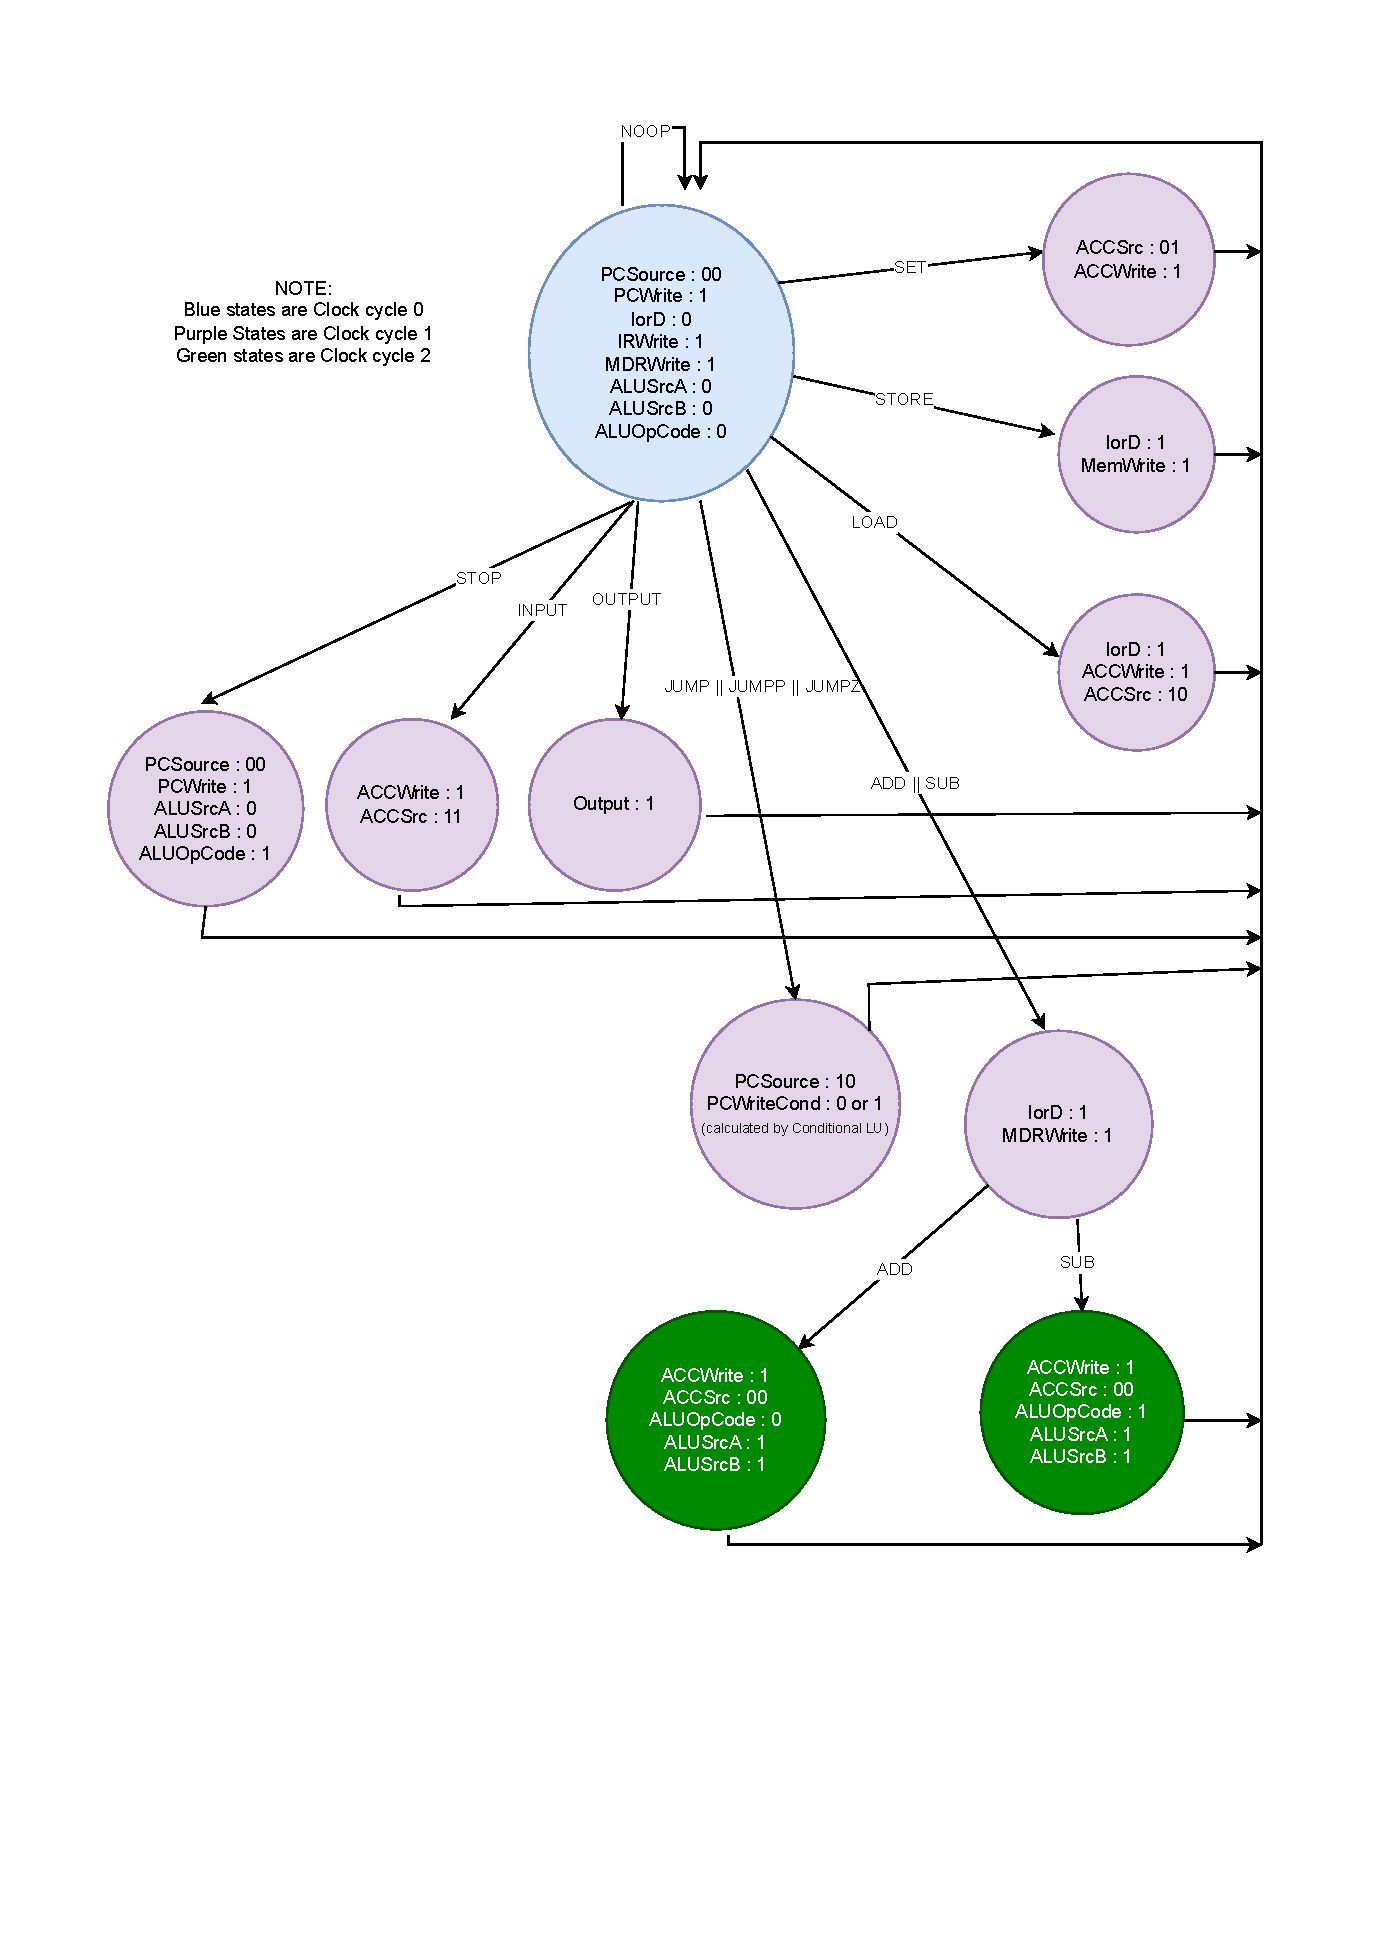
\includepdf[]{VM252FSMWithControlLines.pdf}

\section{Implementing the FSM}
FSM is implemented in the VM252$^*$ with the help of a ROM. The thing to realise is that if we know our current state  with \begin{itemize}
    \item which instruction we are executing
    \item and the clock cycle we are in
\end{itemize}
we can then specify control for that state and also know what the next state should be.
\begin{enumerate}
    \item Our ROM has addresses which are 14-bits long each of which holds value 15-bits long.
    \item The address is made up based on the instruction and the current clock cycle we are in.
    \item A 14-bits address is of the form $a_{13}a_{12}a_{11}a_{10}a_9a_8a_7a_6a_5a_4a_3a_2a_1a_0$ where \begin{itemize}
        \item $a_{13}$ is 1 if OPCODE = INPUT, 0 otherwise
        \item $a_{12}$ is 1 if OPCODE = OUTPUT, 0 otherwise
        \item $a_{11}$ is 1 if OPCODE = NOOP, 0 otherwise
        \item $a_{10}$ is 1 if OPCODE = STOP, 0 otherwise
        \item $a_{9}$ is 1 if OPCODE = LOAD, 0 otherwise
        \item $a_{8}$ is 1 if OPCODE = STORE, 0 otherwise
        \item $a_{7}$ is 1 if OPCODE = ADD, 0 otherwise
        \item $a_{6}$ is 1 if OPCODE = SUB, 0 otherwise
        \item $a_{5}$ is 1 if OPCODE = JUMP, 0 otherwise
        \item $a_{4}$ is 1 if OPCODE = JUMPZ, 0 otherwise
        \item $a_{3}$ is 1 if OPCODE = JUMPP, 0 otherwise
        \item $a_{2}$ is 1 if OPCODE = SET, 0 otherwise
        \item $a_{1}$ and $a_{0}$ form the current clock cycle number for the instruction where $a_{1}$ is the significant bit.
    \end{itemize}
    \item The value of each cell specifies the control lines for the current state and also provides the next clock cycle which is stored in a register so that it can then be used to form the address in the next clock cycle.
    \item A 15-bit value is of the form $v_{14}v_{13}v_{12}v_{11}v_{10}v_9v_8v_7v_6v_5v_4v_3v_2v_1v_0$ such that \begin{itemize}
        \item PCSource : $v_{14}v_{13}$
        \item PCWrite : $v_{12}$
        \item IorD : $v_{11}$
        \item MemWrite : $v_{10}$
        \item IRWrite : $v_{9}$
        \item MDRWrite : $v_{8}$
        \item ACCSrc : $v_{7}v_{6}$
        \item ACCWrite : $v_{5}$
        \item ALUSrcA : $v_{4}$
        \item ALUSrcB : $v_{3}$
        \item Output : $v_{2}$
        \item $v_{1}$ and $v_{0}$ form the next clock cycle number for the instruction where $v_{1}$ is the significant bit.
    \end{itemize}
    \item This helps us implement the FSM.
\end{enumerate}
All the used addresses and their values along with their respective instructions are shown below:
\begin{center}
\begin{tabular}{ |c|c|c|c|c| } 
 \hline
 Instruction & 14 bits Address & Address in hex & 15 bits Value & Value in hex \\
 \hline
 Beg. of Program & 00001000000000 & 0200 & 001001100000001 & 1301 \\
 LOAD & 00001000000001 & 0201 & 000100010100010 & 08A2 \\
LOAD & 00001000000010 & 0202 & 001001100000001 & 1301 \\
 INPUT & 10000000000001 & 2001 & 000000011100010 & 00E2 \\
INPUT & 10000000000010 & 2002 & 001001100000001 & 1301 \\
NOOP & 00100000000001 & 0801 & 001001100000001 & 1301 \\
 OUTPUT & 01000000000001 & 1001 & 000000000000110 & 0006 \\
OUTPUT & 01000000000010 & 1002 & 001001100000001 & 1301 \\
STOP & 00010000000001 & 0401 & 001000000000010 & 1002 \\
STOP & 00010000000010 & 0402 & 001001100000001 & 1301 \\
SET & 00000000000101 & 0005 & 000000001100010 & 0062 \\
SET & 00000000000110 & 0006 & 001001100000001 & 1301 \\
STORE & 00000100000001 & 0101 & 000110000000010 & 0C02 \\
STORE & 00000100000010 & 0102 & 001001100000001 & 1301 \\
JUMP & 00000000100001 & 0021 & 100000000000010 & 4002 \\
JUMP & 00000000100010 & 0022 & 001001100000001 & 1301 \\
JUMPZ & 00000000010001 & 0011 & 100000000000010 & 4002 \\
JUMPZ & 00000000010010 & 0012 & 001001100000001 & 1301 \\
JUMPP & 00000000001001 & 0009 & 100000000000010 & 4002 \\
JUMPP & 00000000001010 & 000A & 001001100000001 & 1301 \\
ADD & 00000010000001 & 0081 & 000100100000010 & 0902 \\
ADD & 00000010000010 & 0082 & 000000000111011 & 003B \\
ADD & 00000010000011 & 0083 & 001001100000001 & 1301 \\
SUB & 00000001000001 & 0041 & 000100100000010 & 0902 \\
SUB & 00000001000010 & 0042 & 000000000111011 & 003B \\
SUB & 00000001000011 & 0043 & 001001100000001 & 1301 \\
 \hline
\end{tabular}
\end{center}


\section{How to run programs?}
\begin{itemize}
    \item Download the VM252.circ, VM252ControlUnit if you haven't already.
    \item Open VM252.circ with logisim and navigate to the \textit{MultiClockCycleVM252} circuit which is the main circuit.
    \item Initialise the Control Unit ROM if it hasn't been initialized already. To do so, right-click on the ROM $\rightarrow$ Select "Load image" $\rightarrow$ Select VM252ControlUnit
    \item Select a program to run as follows:
    \begin{itemize}
        \item You can either write your own program by modifying the VM252 memory. Make sure to properly encode instructions.
        \item Or, you can load up some programs from the \textit{programs} directory. To do so, right-click on the memory $\rightarrow$ Select "Load image" $\rightarrow$ Select a valid program from the \textit{programs} folder.
    \end{itemize}
\end{itemize}
\end{document}
